\section{Finger}

\subsection{Kleberdosierung}
	

	
\subsection{Temperaturtest}
\subsection{Ablöserichtung}


\section{PDMS}

	\begin{figure}[h]
		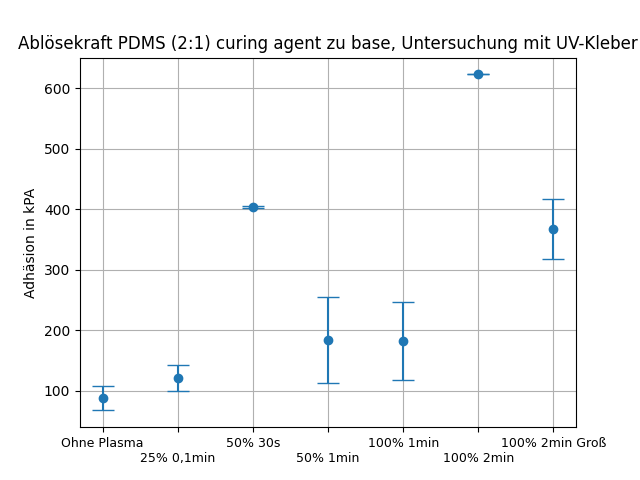
\includegraphics[width=14cm]{test}
		\caption{PDMS 2:1 vergleich bei verschiedenen Plasmacuring stärken und längen.}
	\end{figure}

\section{Lipide}


\begin{figure}[h]
	\begin{tabular}{|c|c|c|c|c|}
		\hline
		Lipide & 4-Methyl Pentene & 3-Methyl Pentene & 1-Pentene & Isopentane \\
		\hline
		EGG-PC & Ja & Geht & Nein & Nein \\
		\hline
		DOPC & ? & Nein & Nein & Geht \\
		\hline
	\end{tabular}
	\begin{tabular}{|c|c|c|c|}
		\hline
		Lipide &  1-Propanol & Pentane & Ethanol \\
		\hline
		EGG-PC & Ja & Ja & ? \\
		\hline
		DOPC & Ja & Nein & Ja \\
		\hline
	\end{tabular}
	\caption{Getestete Lipide und Lösungsmittel unter Raumtemperaturen}
\end{figure}

